\chapter{谱聚类}
谱聚类是从图论中演化出来的算法,后来在聚类中得到了广泛的应用。它的主要思想是把所有的数据看做空间中的点,这些点之间可以用边连接起来。点和点之间的相似度以边的权重形式体现,相似度越高权重越高。通过对所有数据点组成的图进行切图,让切图后不同的子图间边权重和尽可能的低,而子图内的边权重和尽可能的高,从而达到聚类的目的。本节我们首先介绍该问题的相关背景然后在介绍相关加速算法。
\section{谱聚类引入及背景}
由于谱聚类是基于图论的,因此我们首先温习下图的概念。

\subsection{图的概念}
对于一个图$G$,我们一般用点的集合$V$和边的集合$E$来描述。即为$G(V,E)$。其中$V$即为我们数据集里面所有的点$(v_1, v_2,...v_n)$。对于$V$中的任意两个点$v_i,v_j$,我们定义$w_{ij}$为它们之间的边的权重。谱聚类切割的图是无向图,所以$w_{ij}=w_{ji}$。
        
任意$w_{ij}\geq 0$,如果两个点不相似,$w_{ij} = 0$。对于图中的任意一个点$v_i$,它的度$d_i$定义为和它相连的所有边的权重之和,即
\begin{equation*}
d_i = \sum\limits_{j=1}^{n}w_{ij}
\end{equation*}
利用每个点度的定义,我们可以得到一个$n\times n$的度矩阵$D$,它是一个对角矩阵,只有主对角线有值,对应第$i$行的第$i$个点的度数,定义如下:
\begin{equation*}
    D =
  \begin{pmatrix}
    d_{1} & & \\
    & \ddots & \\
    & & d_{n}
  \end{pmatrix}
\end{equation*}
根据所有点间的权重值,我们可以得到图的邻接矩阵$W$,因为$W$反映了两个点的相似度,我们也把$W$称为相似度矩阵。它也是一个$n\times n$的矩阵,第$i$行的第$j$个值对应权重$w_{ij}$。
除此之外,对于点集$V$的的一个子集$A \subset V$,我们定义:
\begin{align*}
& |A|: = \text{子集A中点的个数} \\
& vol(A): = \sum\limits_{i \in A}d_i
\end{align*}

\subsection{相似度矩阵的构建}
在上一节我们讲到了邻接矩阵$W$,它是由任意两点之间的权重值$w_{ij}$组成的矩阵。通常我们可以自己输入权重,但是在谱聚类中,我们只有数据点的定义,并没有直接给出这个邻接矩阵,那么怎么得到这个邻接矩阵呢?

基本思想是,距离较远的两个点之间的边权重值较低,而距离较近的两个点之间的边权重值较高,不过这仅仅是定性,我们需要定量的计算。一般来说,构建邻接矩阵$W$的方法有三类。$\epsilon$-邻近法,$k$邻近法和全连接法。

对于$\epsilon$-邻近法,它设置了一个距离阈值$\epsilon$,然后用欧式距离度量任意两点$x_i$和$x_j$的距离。即令$s_{ij} = ||x_i-x_j||_2^2$,  然后根据$s_{ij}$和$\epsilon$的大小关系,来定义邻接矩阵$W$如下:
\begin{equation*}
w_{ij}= \begin{cases} 0& {s_{ij} > \epsilon}\\ \epsilon& {{s_{ij} \leq \epsilon}} \end{cases}
\end{equation*}
从上式可见,两点间的权重要不就是$\epsilon$,要不就是0,没有其他的信息了。距离远近度量很不精确,因此在实际应用中,我们很少使用$\epsilon$-邻近法。

第二种定义邻接矩阵$W$的方法是$k$邻近法,利用KNN算法遍历所有的样本点,取每个样本最近的$k$个点作为近邻,只有和样本距离最近的$k$个点之间的$w_{ij}>0$。但是这种方法会造成重构之后的邻接矩阵$W$非对称,我们后面的算法需要对称邻接矩阵。为了解决这种问题,一般采取下面两种方法之一,
第一种$k$邻近法是只要一个点在另一个点的$k$近邻中,则计算$w_{ij}$
\begin{equation*}
w_{ij}=w_{ji}= \begin{cases} 0& {x_i \notin KNN(x_j) \;and \;x_j \notin KNN(x_i)}\\ exp(-\frac{||x_i-x_j||_2^2}{2\sigma^2})& {x_i \in KNN(x_j)\; or\; x_j \in KNN(x_i}) \end{cases}
\end{equation*}
第二种$k$邻近法是必须两个点互为$k$近邻中,才计算$w_{ij}$
\begin{equation*}
w_{ij}=w_{ji}= \begin{cases} 0& {x_i \notin KNN(x_j) \;or\;x_j \notin KNN(x_i)}\\ exp(-\frac{||x_i-x_j||_2^2}{2\sigma^2})& {x_i \in KNN(x_j)\; and \; x_j \in KNN(x_i}) \end{cases}
\end{equation*}

第三种定义邻接矩阵$W$的方法是全连接法,相比前两种方法,第三种方法所有的点之间的权重值都大于0,因此称之为全连接法。可以选择不同的核函数来定义边权重,常用的有多项式核函数,高斯核函数和Sigmoid核函数。最常用的是高斯核函数RBF:
\begin{equation*}
w_{ij}=exp(-\frac{||x_i-x_j||_2^2}{2\sigma^2})
\end{equation*}
在实际的应用中,使用第三种全连接法来建立邻接矩阵是最普遍的。

\subsection{拉普拉斯矩阵}
单独把拉普拉斯矩阵(Graph Laplacians)拿出来介绍是因为后面的算法和这个矩阵的性质息息相关。它的定义很简单,拉普拉斯矩阵$L=D-W$。D即为我们第二节讲的度矩阵,它是一个对角矩阵。而$W$即为我们第二节讲的邻接矩阵,它可以由我们第三节的方法构建出。

拉普拉斯矩阵有一些很好的性质如下:
\begin{enumerate}
    \item 拉普拉斯矩阵是对称矩阵,这可以由$D$和$W$都是对称矩阵而得。
    \item 由于拉普拉斯矩阵是对称矩阵,则它的所有的特征值都是实数。
    \item 对于任意的向量$f$,我们有
    \begin{equation*}
    f^TLf = \frac{1}{2}\sum\limits_{i,j=1}^{n}w_{ij}(f_i-f_j)^2
    \end{equation*}
    证明如下
    \begin{equation*}
    f^TLf = f^TDf - f^TWf = \sum\limits_{i=1}^{n}d_if_i^2 - \sum\limits_{i,j=1}^{n}w_{ij}f_if_j
    \end{equation*}
    \begin{equation*}
    =\frac{1}{2}( \sum\limits_{i=1}^{n}d_if_i^2 - 2 \sum\limits_{i,j=1}^{n}w_{ij}f_if_j + \sum\limits_{j=1}^{n}d_jf_j^2) = \frac{1}{2}\sum\limits_{i,j=1}^{n}w_{ij}(f_i-f_j)^2
    \end{equation*}
    \item 拉普拉斯矩阵是半正定的,且对应的n个实数特征值都大于等于0,即$0 =\lambda_1 \leq \lambda_2 \leq... \leq \lambda_n$, 且最小的特征值为0,这个由性质3很容易得出。
\end{enumerate}

\subsection{图切割}
        
对于无向图G的切图,我们的目标是将图$G(V,E)$切成相互没有连接的k个子图,每个子图点的集合为:$A_1,A_2,..A_k$,它们满足$A_i \cap A_j = \emptyset$,且$A_1 \cup A_2 \cup ... \cup A_k = V$.

对于任意两个子图点的集合$A, B \subset V$, $A \cap B =  \emptyset$, 我们定义A和B之间的切图权重为:
\begin{equation*}
W(A, B) = \sum\limits_{i \in A, j \in B}w_{ij}
\end{equation*}
那么对于我们k个子图点的集合:$A_1,A_2,..A_k$,我们定义切图cut为:
\begin{equation*}
cut(A_1,A_2,...A_k) = \frac{1}{2}\sum\limits_{i=1}^{k}W(A_i, \overline{A}_i )
\end{equation*}
其中$\bar{A_i}$为$A_i$的补集,意为$V - A_i$。

那么如何切图可以让子图内的点权重和高,子图间的点权重和低呢?一个自然的想法就是最小化$cut(A_1,A_2,...A_k)$, 但是可以发现,这种极小化的切图存在问题,如图1所示,
\begin{figure}[h]
    \centering
    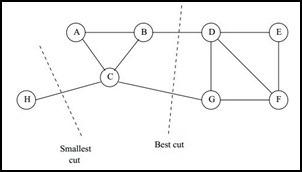
\includegraphics[scale=0.7]{cut_problem.jpg}
    \caption{可能出现的不好的切割}
\end{figure}
我们选择一个权重最小的边缘的点,比如$C$和$H$之间进行cut,这样可以最小化$cut(A_1,A_2,...A_k)$, 但是却不是最优的切图,如何避免这种切图,并且找到类似图中"Best Cut"这样的最优切图呢?我们下一节就来看看谱聚类中常用的切图方法。

\subsection{Normalized Cut}
为了避免最小切图导致的切图效果不佳,我们需要对每个子图的规模做出限定,一般来说,有两种切图方式,第一种是RatioCut,第二种是Ncut。一般我们使用Ncut,故在此只介绍Ncut。

Normalized cut切图为了避免上一节中的不好的切图,对每个切图,不光考虑最小化$cut(A1,A2,...Ak)$,它还同时考虑每个类中点的数目尽可能平衡,即
\begin{equation*}
NCut(A_1,A_2,...A_k) = \frac{1}{2}\sum\limits_{i=1}^{k}\frac{W(A_i, \overline{A}_i )}{vol(A_i)}
\end{equation*}
为了优化该目标函数,我们定义如下指示向量。
\begin{equation*}
h_{ij}= \begin{cases} 0& { v_i \notin A_j}\\ \frac{1}{\sqrt{vol(A_j)}}& { v_i \in A_j} \end{cases}
\end{equation*}
则
对于$h_i^TLh_i$,有:
\begin{align} h_i^TLh_i & = \frac{1}{2}\sum\limits_{m=1}\sum\limits_{n=1}w_{mn}(h_{im}-h_{in})^2 \\& =\frac{1}{2}(\sum\limits_{m \in A_i, n \notin A_i}w_{mn}(\frac{1}{\sqrt{vol(A_i)}} - 0)^2 +  \sum\limits_{m \notin A_i, n \in A_i}w_{mn}(0 - \frac{1}{\sqrt{vol(A_i)}} )^2\\& = \frac{1}{2}(\sum\limits_{m \in A_i, n \notin A_i}w_{mn}\frac{1}{vol(A_i)} +  \sum\limits_{m \notin A_i, n \in A_i}w_{mn}\frac{1}{vol(A_i)}\\& = \frac{1}{2}(cut(A_i, \overline{A}_i) \frac{1}{vol(A_i)} + cut(\overline{A}_i, A_i) \frac{1}{vol(A_i)}) \\& =  \frac{cut(A_i, \overline{A}_i)}{vol(A_i)} 
\end{align}
也就是说
\begin{equation*}
NCut(A_1,A_2,...A_k) = \sum\limits_{i=1}^{k}h_i^TLh_i = \sum\limits_{i=1}^{k}(H^TLH)_{ii} = tr(H^TLH)
\end{equation*}
我们将Ncut的优化问题转化为了一个二次型优化问题,并注意到该问题有如下限制
\begin{equation*}
h_i^TDh_i = \sum\limits_{j=1}^{n}h_{ij}^2d_j =\frac{1}{vol(A_i)}\sum\limits_{j \in A_i}d_j= \frac{1}{vol(A_i)}vol(A_i) =1
\end{equation*}
此时,我们得到如下优化问题
\begin{equation*}
\argmin\limits_{H} \; tr(H^TLH) \;\; s.t.\;H^TDH=I
\end{equation*}
注意到$H$是离散的,此时该问题是NP难的,为了求解我们允许$H$可以取连续值,该步骤称为relaxation,
使用拉格朗日乘子法可以求解,解为$D^{-1/2}LD^{-1/2}$的最小的前k个特征值,对应的$H$为$D^{-1/2}LD^{-1/2}$的前k个特征向量,对H的每一行再做聚类,比如k-means即可得到最后的聚类结果。